\documentclass[letterpaper]{article}
\usepackage{amssymb}
\usepackage{fullpage}
\usepackage{amsmath}
\usepackage{epsfig,float,alltt, epstopdf}
\usepackage{psfrag,xr}
\usepackage[T1]{fontenc}
\usepackage{url}
%\usepackage{mathtools}

\begin{document}

\newcommand{\trace}{\mathrm{trace}}
\newcommand{\real}{\mathbb R}  % real numbers  {I\!\!R}
\newcommand{\nat}{\mathbb R}   % Natural numbers {I\!\!N}
\newcommand{\cp}{\mathbb C}    % complex numbers  {I\!\!\!\!C}
\newcommand{\ds}{\displaystyle}
\newcommand{\mf}[2]{\frac{\ds #1}{\ds #2}}
\newcommand{\book}[2]{{Luenberger, Page~#1, }{Prob.~#2}}
\newcommand{\spanof}[1]{\textrm{span} \{ #1 \}}
\parindent 0pt


\begin{center}
{\large \bf HW \# 05 Solutions}
\end{center}

\vspace*{1cm}

%Prob. 1 Inner Products
\noindent \textbf{Problem  1:}
\begin{enumerate}
\setlength{\itemsep}{.1in}
\renewcommand{\labelenumi}{(\alph{enumi})}
\item $\begin{aligned}<x,y> = x^\top \bar{y} = \sum_{i=1}^{n} x_i \bar{y}_i \end{aligned}\;$.
\begin{enumerate}
\setlength{\itemsep}{.1in}
\renewcommand{\labelenumii}{(\roman{enumii})}
\item $\begin{aligned}[t] \overline{<y, x>} &= \overline{y^\top \bar{x}}=\overline{\sum_{i=1}^{n}y_i \bar{x}_i} = \sum_{i=1}^{n}\bar{y}_ix_i \\ & = <x,y>. \end{aligned}$

\item $\begin{aligned}[t] <\alpha_1 x_1+\alpha_2 x_2, y> & =(\alpha_1 x_1+\alpha_2 x_2)^\top \bar{y} \\&=\alpha_1x_1^\top\bar{y}+\alpha_2 x_2^\top\bar{y} \\ &=\alpha_1<x_1,y>+\alpha_2<x_2,y>.\end{aligned} $

\item $\begin{aligned}<x,x>=\sum_{i=1}^n x_i \bar{x}_i=\sum_{i=1}^n |x_i|^2\end{aligned}$.
\smallskip \\
Hence, $<x, x> \geq 0$ for any $x\in \cp^n$, and $<x, x> = 0 \iff |x_i|^2=0, i = 1, ..., n, \iff x=0$.
\end{enumerate}

\item $\begin{aligned} <x,y> = \bar{x}^\top y = \sum_{i=1}^{n}\bar{x}_i y_i\; .\end{aligned}$
\begin{enumerate}
\setlength{\itemsep}{.1in}
\renewcommand{\labelenumii}{(\roman{enumii})}
\item $\begin{aligned}[t]\overline{<y,x>} &= \overline{\bar{y}^\top x}=\overline{\sum_{i=1}^n \bar{y}_i x_i} \\
&=\sum_{i=1}^n y_i \bar{x}_i = \bar{x}^\top y = <x,y>.\end{aligned}$

\item $\begin{aligned}[t]<x, \beta_1 y_1+\beta_2 y_2> &= \bar{x}^\top(\beta_1 y_1+\beta_2 y_2)\\
& = \beta_1 \bar{x}^\top y_1+\beta_2 \bar{x}^\top y_2 \\
& = \beta_1<x, y_1>+\beta_2<x, y_2>. \end{aligned}$

\item $\begin{aligned}[t]<x, x> = \bar{x}^\top x = \sum_{i=1}^n \bar{x}_i x_i = \sum_{i=1}^n |x_i|^2.\end{aligned}$
\smallskip \\
Hence, $<x,x>\geq 0$ for any $x \in \cp^n$, and $<x,x>=0 \iff |x_i|^2 = 0, i = 1, ..., n, \iff x=0$
\end{enumerate}
\end{enumerate}

%Prob. 2 Legendre Polynomials
\noindent \textbf{Problem  2:}
$$<f, g> = \int_{-1}^1 f(x)g(x)dx$$
$$\begin{aligned}\textbf{\textit{p}}_0(x)&=1,~~\textbf{\textit{p}}_2(x)=\frac{1}{2}(3x^2-1) \\
\textbf{\textit{p}}_1(x)&=x,~~\textbf{\textit{p}}_4(x)=\frac{1}{2}(5x^3-3x).\end{aligned}$$

$$\begin{aligned}<\textbf{\textit{p}}_0, \textbf{\textit{p}}_3> &=\int_{-1}^{1}\textbf{\textit{p}}_0(x)\textbf{\textit{p}}_3(x)dx\\
&=\int_{-1}^{1}\frac{1}{2}(5x^3-3x)dx\\
&=\frac{1}{2}\bigg[\frac{5x^4}{4}-\frac{3x^2}{2}\bigg]\bigg|_{-1}^1\\
&=\frac{1}{2}\bigg[(\frac{5}{4}-\frac{3}{2})-(\frac{5}{4}-\frac{3}{2})\bigg]\\
&=0.\end{aligned}$$

$$\begin{aligned}<\textbf{\textit{p}}_1, \textbf{\textit{p}}_2> &=\int_{-1}^{1}\textbf{\textit{p}}_1(x)\textbf{\textit{p}}_2(x)dx\\
&=\int_{-1}^{1}x\frac{1}{2}(3x^2-1)dx\\
&=\int_{-1}^{1}\frac{1}{2}(3x^3-x)dx\\
&=\frac{1}{2}\bigg[\frac{3x^4}{4}-\frac{x^2}{2}\bigg]\bigg|_{-1}^1\\
&=\frac{1}{2}\bigg[(\frac{3}{4}-\frac{1}{2})-(\frac{3}{4}-\frac{1}{2})\bigg]\\
&=0.\end{aligned}$$

%Prob. 3 Orthogonal vectors, GS
\noindent \textbf{Problem  3:}
$$\begin{aligned} v^1 &= y^1 = \begin{bmatrix} 1\\ -2\\ 1\end{bmatrix}, ~~\|v^1\|^2 = 6.\\
v^2 &= y^2 - a_{21} v^1.\\
a_{21} &= \frac{<y^2, v^1>}{\|v^1\|^2} = \frac{\left[\begin{array}{ccc} 4& 0& -1\end{array}\right]\begin{bmatrix} 1\\ -2\\ 1\end{bmatrix}}{6},\\
&=\frac{3}{6} = \frac{1}{2}.\end{aligned}$$

$$\therefore v^2 = \begin{bmatrix} 4\\0\\-1\end{bmatrix}-\frac{1}{2}\begin{bmatrix} 1\\-2\\1\end{bmatrix}=\begin{bmatrix}3\dfrac{1}{2}\\[2ex]1\\[2ex]-1\dfrac{1}{2}\end{bmatrix}=\frac{1}{2}\begin{bmatrix}7\\2\\-3\end{bmatrix}.$$

$$\|v^2\|^2 = \frac{1}{4} (49+4+9) = \frac{62}{4} = \frac{31}{2}.$$
\medskip
$$v^3 = y^3 - a_{31}v^1-a_{32}v^2.$$
$$\begin{aligned} a_{31} &= \frac{<y^3, v^1>}{\|v^1\|^2} = \frac{\left[\begin{array}{ccc} -2& 2& 3\end{array}\right]\begin{bmatrix} 1\\ -2\\ 1\end{bmatrix}}{6},\\
&= -\frac{3}{6} = -\frac{1}{2}. \end{aligned}$$

$$\begin{aligned} a_{32} &= \frac{<y^3, v^2>}{\|v^2\|^2} = \frac{\left[\begin{array}{ccc} -2& 2& 3\end{array}\right]\begin{bmatrix} 7\\ 2\\ -3\end{bmatrix}\bigg(\dfrac{1}{2}\bigg)}{3\dfrac{1}{2}},\\ &= -\frac{19}{31}.\end{aligned}$$

$$\begin{aligned}v^3 &= \begin{bmatrix} -2\\ 2\\ 3\end{bmatrix} + \frac{1}{2}\begin{bmatrix} 1\\ -2\\ 1\end{bmatrix} + \frac{19}{31}\begin{bmatrix} 3\dfrac{1}{2}\\[2ex] 1\\[2ex] -1\dfrac{1}{2}\end{bmatrix}\\
&=\begin{bmatrix} 40\\ 100\\ 160\end{bmatrix}(\frac{1}{62})\approx\begin{bmatrix} 0.65\\ 1.61\\ 2.58\end{bmatrix}.\end{aligned}$$

%Prob. 4 Matrix Inversion Lemma
\noindent \textbf{Problem  4:}
\begin{enumerate}
\setlength{\itemsep}{.1in}
\renewcommand{\labelenumi}{(\alph{enumi})}
\item If $A^{-1}$, $C^{-1}$ and $(C^{-1}+DA^{-1}B)^{-1}$ each exist, then
$$M = A^{-1}-A^{-1}B(C^{-1} + DA^{-1}B)^{-1}DA^{-1}~~(*)$$
is well defined (means each of the terms exists and the indicated matrix products are compatible).
\medskip \\
\underline{To show}: The proposed inverse $(*)$ when multiplied by $(A+BCD)$ gives the identity.
\smallskip \\
We will show $M(A+BCD)=I$.
$$\begin{aligned}M(A+BCD) &= I - A^{-1}B(C^{-1} + DA^{-1}B)^{-1}D + A^{-1}BCD - A^{-1}B(C^{-1}+DA^{-1}B)^{-1}DA^{-1}BCD
\\ &= I - A^{-1}B \big[ (C^{-1}+DA^{-1}B)^{-1}C^{-1}-I+(C^{-1}+DA^{-1}B)^{-1}DA^{-1}B \big] CD
\\ &= I - A^{-1}B \big[ (C^{-1}+DA^{-1}B)^{-1}(C^{-1}+DA^{-1}B)-I \big]CD
\\ &= I - A^{-1}B [I-I] D
\\ &= I. \end{aligned}$$

\item $$A^{-1} = \text{diag}([1, 2, 2, 1, 2]),$$
$$C^{-1} = 5,$$
$$A^{-1}B = \begin{bmatrix} 1\\ 0\\ 4\\ 0\\ 6\end{bmatrix},$$
$$DA^{-1}B = \left[\begin{array}{ccccc} 1 & 0 & 2 & 0 & 3 \end{array}\right] \begin{bmatrix} 1\\ 0\\ 4\\ 0\\ 6\end{bmatrix} = 27,$$
$$C^{-1}+DA^{-1}B = 32 \implies (C^{-1}+DA^{-1}B)^{-1} = \frac{1}{32}.$$
$$DA^{-1} = \left[\begin{array}{ccccc} 1 & 0 & 4 & 0 & 6 \end{array}\right],$$
$$\begin{aligned}\therefore (A+BCD)^{-1} &= \left[\begin{array}{ccccc} 1 & 0 & 0 & 0 & 0 \\
0 & 2 & 0 & 0 & 0 \\
0 & 0 & 2 & 0 & 0 \\
0 & 0 & 0 & 1 & 0 \\
0 & 0 & 0 & 0 & 2 \end{array}\right] - \begin{bmatrix} 1\\ 0\\ 4\\ 0\\ 6\end{bmatrix}(\frac{1}{32})\left[\begin{array}{ccccc} 1 & 0 & 4 & 0 & 6\end{array}\right]\\
&= \left[\begin{array}{ccccc} 1 & 0 & 0 & 0 & 0 \\
0 & 2 & 0 & 0 & 0 \\
0 & 0 & 2 & 0 & 0 \\
0 & 0 & 0 & 1 & 0 \\
0 & 0 & 0 & 0 & 2 \end{array}\right] - \frac{1}{32}\left[\begin{array}{ccccc}
1 & 0 & 4 & 0 & 6 \\
0 & 0 & 0 & 0 & 0 \\
4 & 0 & 16 & 0 & 24 \\
0 & 0 & 0 & 0 & 0 \\
6 & 0 & 24 & 0 & 36 \end{array}\right]\\
&= \frac{1}{32}\left[\begin{array}{ccccc}
31 & 0 & -4 & 0 & -6 \\
0 & 64 & 0 & 0 & 0 \\
-4 & 0 & 48 & 0 & -24 \\
0 & 0 & 0 & 32 & 0\\
-6 & 0 & -24 & 0 & 28 \\
\end{array}\right].
\end{aligned}$$
\end{enumerate}


%Prob. 5 Regression no noise
\noindent \textbf{Problem  5:}

\begin{enumerate}
\setlength{\itemsep}{.1in}
\renewcommand{\labelenumi}{(\alph{enumi})}

\item The naive estimate is plotted in Fig. \ref{fig:naive5}
\begin{figure}[h]
\centering
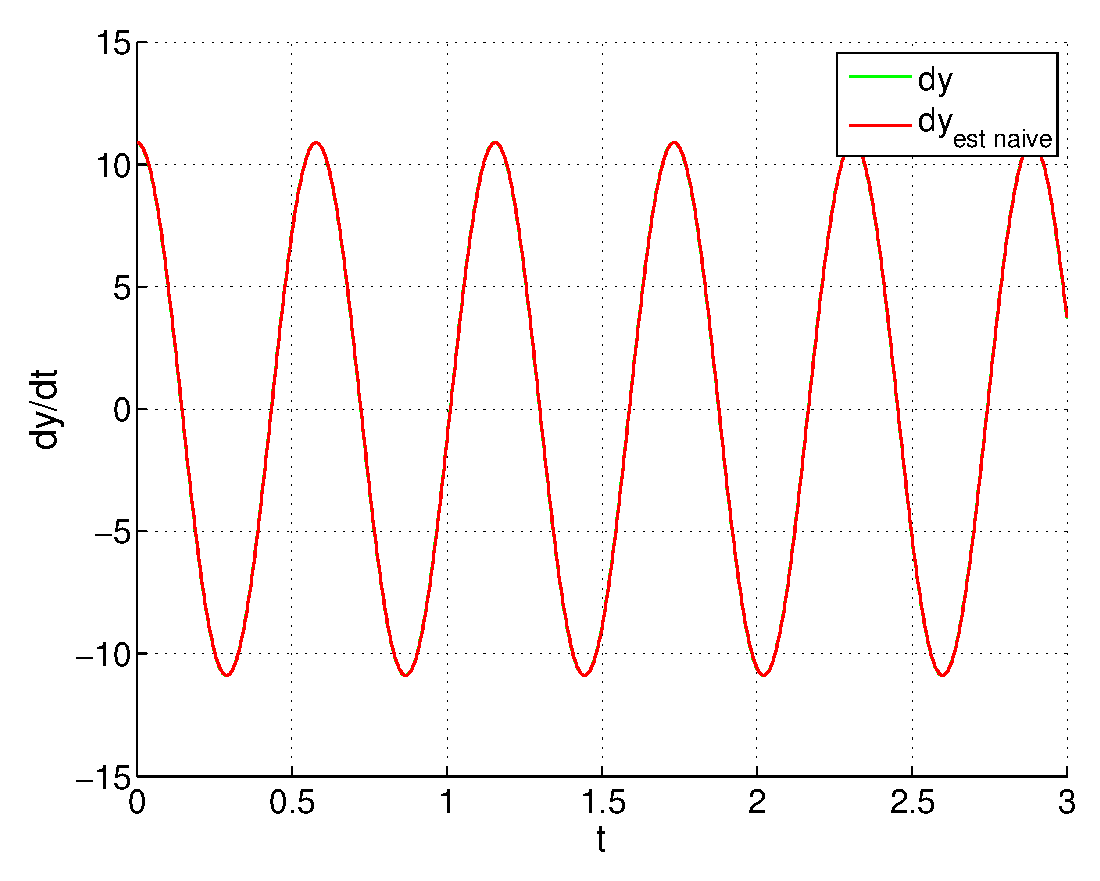
\includegraphics[width=0.6\textwidth]{HW5Pb5_Naive.eps}
\setlength{\abovecaptionskip}{0pt}
\caption{Naive Estimate}\label{fig:naive5}
\end{figure}

\item  We define $Y_k$ so that it contains $M\ge2$ of the ``most recent'' data points
$$Y_k = \left[ \begin{array}{l} y[k-M+1] \\ \vdots \\  y[k] \end{array} \right], $$
where $y[k] = y(k \Delta T)$. For basis functions, we take the monomials, but you can use any set of independent functions for which you can compute the derivative. We let $\varphi_i(t) = t^i$, where $\varphi_0(t) = 1$. \\

 Suppose that at time $t_k=k \Delta T$, we regress the data against  $\{\varphi_0(t), \cdots, \varphi_N(t) \}$, in other words,
$${y}(t) = \alpha_0 + \alpha_1 t+ \cdots +   \alpha_N t^N.$$
We then have
$$Y_k = A_k \alpha$$
where
$$ A_k = \left[ \begin{array}{crcr} 1 & (k-M+1)\Delta T & \cdots &  ( (k-M+1)\Delta T )^N\\
1 & (k-M+2)\Delta T & \cdots &  ( (k-M+2)\Delta T )^N \\
\vdots & \vdots~~~~ & \cdots & \vdots~~~~ \\
1 & (k-2)\Delta T & \cdots &  ((k- 2) \Delta T )^N \\
1 &  (k-1)\Delta T & \cdots &   ((k-1) \Delta T )^N \\
1 & k\Delta T~~ & \cdots &  (k \Delta T)^N~~~~ \\
\end{array} \right] $$
which depends on $k$, and thus changes step-to-step. We need $M\ge N+1$ for the columns of the matrix to be linearly independent. At the $k$-th step we have
$$ \alpha = (A_k^\top A_k)^{-1}A_k^\top Y_k $$
We plug these coefficients back into
$${y}(t) = \alpha_0 + \alpha_1 (t) + \cdots +   \alpha_N (t)^N,$$
we differentiate it, evaluate it at whatever time we desire, and use that for our estimate of $\dot{y}(t)$. This is an acceptable solution, but a much more practical solution is available to us.\\


Suppose instead that at time $t_k$, we regress the data against  $\{\varphi_0(t-t_k), \cdots, \varphi_N(t-t_k) \}$, in other words,
$${y}(t) = \alpha_0 + \alpha_1 (t-t_k) + \cdots +   \alpha_N (t-t_k)^N.$$
All we are doing is shifting the time origin to $t_k$. By doing this, we end up with
$$Y_k = A \alpha$$
where
$$ A = \left[ \begin{array}{crcr} 1 & (-M+1)\Delta T & \cdots &  ( (-M+1)\Delta T )^N\\
1 & (-M+2)\Delta T & \cdots &  ( (-M+2)\Delta T )^N \\
\vdots & \vdots~~~~ & \cdots & \vdots~~~~ \\
1 & -2\Delta T & \cdots &  (- 2\Delta T )^N \\
1 & -\Delta T & \cdots &  (- \Delta T )^N \\
1 & 0~~ & \cdots &  0~~~~ \\
\end{array} \right] $$
which does not change from one time step to the next. We still need $M\ge N+1$ for the columns of the matrix to be linearly independent. At the $k$-th step we have
$$ \alpha = (A^\top A)^{-1}A^\top Y_k $$
and we only need to compute $ (A^\top A)^{-1}A^\top$ once. This is what I do on my robots. The calculation of the inverse is done off-line and stored.\\

We now compute
$$\dot{y}(t) =  \alpha_1 + 2 \alpha_2 (t-t_k)+ \cdots +   N \alpha_N (t-t_k)^{(N-1)},$$
and thus
$$\dot{y}(t) = \left[ 0, 1,  2 (t-t_k), \cdots ,   N  (t-t_k)^{(N-1)} \right] \alpha$$

Setting $t=t_k$, we obtain
$$\widehat{\dot{y}}_k = \left[ 0, 1,  0, \cdots ,   0\right] \alpha, $$
in other words,
$$ \widehat{\dot{y}}_k = R Y_k$$
where $$R=\left[ 0, 1,  0, \cdots ,   0\right]  (A^\top A)^{-1}A^\top.$$
\begin{figure}[h]
\centering
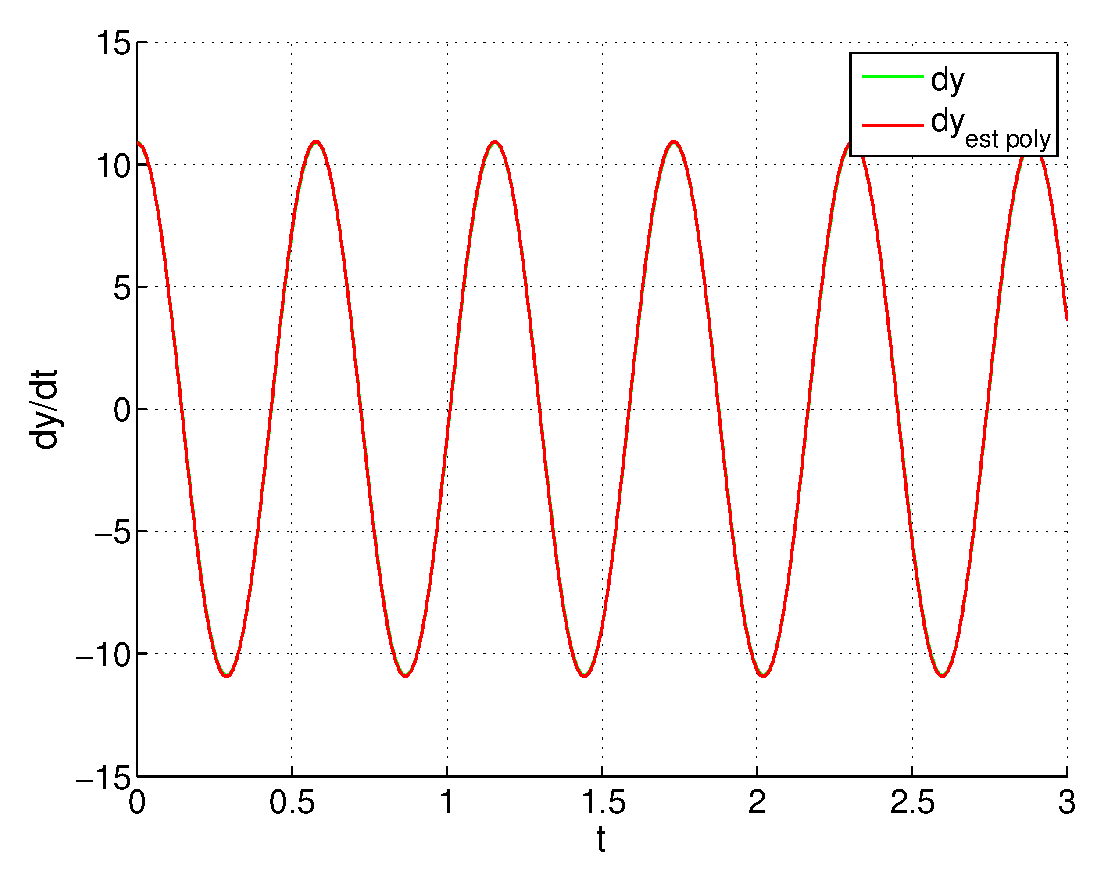
\includegraphics[width=0.6\textwidth]{HW5Pb5_poly.eps}
\setlength{\abovecaptionskip}{0pt}
\caption{Regression}\label{fig:regressPoly5}
\end{figure}

 Choosing $M=4$ and $N=2$, we obtain the plot of the derivative given in Fig. \ref{fig:regressPoly5} It looks exactly that same as the naive derivative, so we are disappointed that we worked so hard! \textbf{Remark: If you take $M=2$ and $N=1$ you get exactly the naive derivative.}

\end{enumerate}

%Prob. 6 Regression noise
\noindent \textbf{Problem  6:}

\begin{enumerate}
\setlength{\itemsep}{.1in}
\renewcommand{\labelenumi}{(\alph{enumi})}

\item The naive estimate is plotted in Fig. \ref{fig:naive6}. Computing the error gives
$$ \frac{|| \dot{y}_k - \widehat{\dot{y}}_k||}{\mbox{Length of the data vector}}  =  0.093,$$
\begin{figure}[h!]
\centering

\includegraphics[width=0.7\textwidth]{Prob06naive.png}
\setlength{\abovecaptionskip}{0pt}
\caption{Naive Estimate}\label{fig:naive6}
\end{figure}
\begin{figure}[h!]
\centering

\includegraphics[width=0.7\textwidth]{Prob06regresPoly.png}
\setlength{\abovecaptionskip}{0pt}
\caption{Regression}\label{fig:regressPoly6}
\end{figure}
\item We do the same regression analysis as in Problem 5. We play around with the parameters a bit and settle on $M=10$ and $N=2$. We obtain
$$ \frac{|| \dot{y}_k - \widehat{\dot{y}}_k||}{\mbox{Length of the data vector}}  =  0.027,$$
and a plot of the derivative is given in Fig. \ref{fig:regressPoly6}
\end{enumerate}



% 7 Normal Equations
\noindent \textbf{Problem  7:}
We apply the normal equations:
$$\hat{x} = \alpha_1y^1+\alpha_2y^2,$$
where $G^\top\alpha = b$ and
$$\begin{aligned} G &= \left[\begin{array}{cc}
<y^1, y^1> & <y^2, y^1>\\
<y^1, y^2> & <y^2, y^2>\end{array}\right],\\
b &= \begin{bmatrix}<x, y^1> \\ <x, y^2>\end{bmatrix}.\end{aligned}$$
Doing the calculations, we have
$$<y^1, y^1> = \mathrm{tr}\bigg(\left[\begin{array}{cc}1 & 2\\ 0 & 0\end{array}\right]\left[\begin{array}{cc}1 & 0\\ 2 & 0\end{array}\right]\bigg) = \mathrm{tr}\bigg(\left[\begin{array}{cc}5 & 0\\ 0 & 0\end{array}\right]\bigg) = 5.$$

$$<y^1, y^2> = <y^2, y^1> = \mathrm{tr}\bigg(\left[\begin{array}{cc}1 & 2\\ 0 & 0\end{array}\right]\left[\begin{array}{cc}1 & 1\\ 1 & 1\end{array}\right]\bigg) = \mathrm{tr}\bigg(\left[\begin{array}{cc}3 & 3\\ 0 & 0\end{array}\right]\bigg) = 3.$$

$$<y^2, y^2> = \mathrm{tr}\bigg(\left[\begin{array}{cc}1 & 1\\ 1 & 1\end{array}\right]\left[\begin{array}{cc}1 & 1\\ 1 & 1\end{array}\right]\bigg) = \mathrm{tr}\bigg(\left[\begin{array}{cc}2 & 2\\ 2 & 2\end{array}\right]\bigg) = 4.$$

$$<x, y^1> = \mathrm{tr}\bigg(\left[\begin{array}{cc}0 & 2\\ -1 & 0\end{array}\right]\left[\begin{array}{cc}1 & 0\\ 2 & 0\end{array}\right]\bigg) = \mathrm{tr}\bigg(\left[\begin{array}{cc}4 & 0\\ -1 & 0\end{array}\right]\bigg) = 4.$$

$$<x, y^2> = \mathrm{tr}\bigg(\left[\begin{array}{cc}0 & 2\\ -1 & 0\end{array}\right]\left[\begin{array}{cc}1 & 1\\ 1 & 1\end{array}\right]\bigg) = \mathrm{tr}\bigg(\left[\begin{array}{cc}2 & 2\\ -1 & -1\end{array}\right]\bigg) = 1.$$

$$\therefore \left[\begin{array}{cc}5 & 3\\ 3 & 4\end{array}\right]\begin{bmatrix} \alpha_1 \\ \alpha_2 \end{bmatrix} = \begin{bmatrix} 4 \\ 1\end{bmatrix}.$$

$$\therefore \begin{bmatrix} \alpha_1 \\ \alpha_2 \end{bmatrix} = \frac{1}{11}\left[\begin{array}{cc} 4 & -3 \\ -3 & 5 \end{array}\right] \begin{bmatrix} 4 \\ 1\end{bmatrix} = \frac{1}{11} \begin{bmatrix} 13 \\ -7 \end{bmatrix} = \begin{bmatrix} 1.18 \\ -0.64 \end{bmatrix}.$$

$$\hat{x} = \frac{13}{11} \left[\begin{array}{cc} 1 & 0 \\ 2 & 0 \end{array}\right] - \frac{7}{11} \left[\begin{array}{cc} 1 & 1 \\ 1 & 1 \end{array}\right] = \left[\begin{array}{cc} \strut\dfrac{6}{11} & -\strut\dfrac{7}{11} \\[2.5ex] \strut\dfrac{19}{11} & -\strut\dfrac{7}{11} \end{array}\right].$$
\medskip\\
% 8 Strictly normed
\noindent \textbf{Problem  8:}
Let $\gamma := d(x, M)$, and suppose that $m_1, m_2 \in M$ satisfy $\|x - m_i \| = \gamma$.
\smallskip \\
\underline{To Show} $m_1 = m_2$ when the norm is strict.\smallskip \\
Because $M$ is a subspace, $\frac{m_1 + m_2}{2} \in M$.
\smallskip \\
Hence,
$$\begin{aligned} \gamma &= \inf_{y\in M} ||x-y|| \leq \bigg\|x-\frac{m_1 + m_2}{2}\bigg\| \\
&= \bigg\|\frac{x-m_1}{2}+\frac{x-m_2}{2}\bigg\| \\
&\leq \frac{1}{2}||x-m_1|| + \frac{1}{2}||x-m_2|| \\
& = \frac{\gamma}{2} + \frac{\gamma}{2} \\
& = \gamma. \end{aligned}$$
Hence, $||(x-m_1)+(x-m_2)|| = ||x-m_1|| + ||x-m_2||.$
\smallskip \\
Because the norm is strict, $\exists \alpha \geq 0$ such that either
\begin{enumerate}
\setlength{\itemsep}{.1in}
\renewcommand{\labelenumi}{(\roman{enumi})}
\item $(x-m_1) = \alpha (x-m_2)~~$ or

\item $(x-m_2) = \alpha (x-m_1).$
\end{enumerate}
In either case, we deduce from $\gamma = ||x-m_1|| = ||x-m_2||$, that $\gamma = \alpha \gamma$, and, because $\gamma \neq 0$, we have $\alpha = 1$.
\smallskip \\
With $\alpha = 1$, we have $x-m_1 = x-m_2$, and thus $m_1 = m_2$. $\hfill \square$
\medskip \\

% 9 Strictly normed
\noindent \textbf{Problem  9:}
\begin{enumerate}
\setlength{\itemsep}{.1in}
\renewcommand{\labelenumi}{(\alph{enumi})}
\item \underline{Not strictly normed.} Let
$$x = \begin{bmatrix} 1 \\ 0 \end{bmatrix} ~~ \text{and} ~~ y = \begin{bmatrix} 0 \\ 1 \end{bmatrix}.$$
Then $||x+y||_1 = 2 = ||x||_1 + ||y||_1$, but there does not exist any $\alpha \geq 0$ such that either $x = \alpha y$ or $y = \alpha x$.

\item[(c)] \underline{Not strictly normed.} Let
$$x = \begin{bmatrix} 2 \\ 1 \end{bmatrix} ~~ \text{and} ~~ y = \begin{bmatrix} 4 \\ 1 \end{bmatrix}.$$
Then $6 = ||x+y||_\infty = ||x||_\infty + ||y||_\infty$, but there does not exist any $\alpha \geq 0$ such that either $x = \alpha y$ or $y = \alpha x$.

\item[(b)] \underline{Strictly normed.} The result is true for any norm induced by an inner product. Hence we give the proof for $||x|| = <x, x>^{1/2}.$
\medskip \\
Let $x, y \in X$
\medskip \\
\underline{Case 1} Either $x$ or $y$ is zero. Then $||x+y|| = ||x||+||y||$ is always true and either $x = 0\cdot y$ or $y = 0 \cdot x$ holds. $\hfill \square$

\underline{Case 2} Both $x \neq 0$ and $y \neq 0$, but $\{x, y\}$ is linearly dependent. Then $x = \alpha y$ for some $\alpha \in \real$. It follows that $||x+y|| = ||1+\alpha||\cdot||y||$ and $||x||+||y|| = (1+|\alpha|)||y||$. Because $y \neq 0$, we have
$$||x+y|| = ||x||+||y|| \iff |1+\alpha| = 1+|\alpha| \iff \alpha \geq 0.$$
Hence, $||x+y|| = ||x||+||y|| \iff x = \alpha y, \alpha \geq 0$.
$\hfill \square$

\underline{Case 3} $\{x, y\}$ is linearly independent. By the Gram-Schmidt procedure, there exists $v\in X$ such that $x \perp v$ and $\spanof{x, y} = \spanof{x, v}$. Write $y = \alpha_1x+\alpha_2v$, so that
$$\begin{aligned}[t]& x+y = (1+\alpha_1)x+\alpha_2 v\;, ~~ ||x+y|| = ||x||+||y||~~ \\ &\text{if, and only if,}
||x+y||^2 = ||x||^2+||y||^2+2||x||\cdot||y||\end{aligned}$$
By the Pythagorean Theorem,
$$\begin{aligned}||x+y||^2 &= ||(1+\alpha_1)x+\alpha_2v||^2\\
&= (1+\alpha_1)^2||x||^2+(\alpha_2)^2||v||^2\\
&= [1+2\alpha_1+(\alpha_1)^2]||x||^2 + (\alpha_2)^2||v||^2.\end{aligned}$$
Furthermore
$$||y||^2 = (\alpha_1)^2 ||x||^2 + (\alpha_2)^2 ||v||^2.$$
Hence,
$$||x+y||^2 = ||x||^2+||y||^2+2||x||\cdot||y||~~ \text{if, and only if,}~~ 2\alpha_1||x||^2 = 2||x||\cdot||y||.$$
Because $||x||\neq 0$ from $\{x, y\}$ linear independent, we have $$\alpha_1 ||x|| = ||y||.$$
$\therefore \alpha_1 \geq 0$. Moreover,
$$(\alpha_1)^2 ||x||^2 = ||y||^2 = (\alpha_1)^2 ||x||^2 + (\alpha_2)^2 ||v||^2~~ \text{if, and only if,}~~ \alpha_2 = 0.$$
Hence,
$$||x+y|| = ||x||+||y||~~ \text{if, and only if,}~~ y = \alpha_1 x, \alpha_1 \geq 0 $$ $\hfill \square$
\end{enumerate}

\end{document}




